%!TEX root = ../greb.tex
% Тип документа
\documentclass[a4paper,12pt]{extarticle}

% Шрифты, кодировки, символьные таблицы, переносы
% \usepackage{cmap}
% \usepackage[T2A]{fontenc}
\usepackage[utf8]{inputenc}
\usepackage[russian]{babel}
% Это пакет -- хитрый пакет, он нужен но не нужен
\usepackage[mode=buildnew]{standalone}

\usepackage
	{
		% Дополнения Американского математического общества (AMS)
		amssymb,
		amsfonts,
		amsmath,
		amsthm,
		% Пакет для физических текстов
		physics,
		% misccorr,
		% 
		% Графики и рисунки
		wrapfig,
		graphicx,
		subcaption,
		float,
		tikz,
		tikz-3dplot,
		caption,
		csvsimple,
		color,
		booktabs,
		geometry,
		% 
		% Таблицы, списки
		makecell,
		multirow,
		indentfirst,
		%
		% Интегралы и прочие обозначения
		ulem,
		esint,
		esdiff,
		% 
		% Колонтитулы
		fancyhdr,
	} 
    
\usepackage{mathtools}
\mathtoolsset{showonlyrefs=true} 
\usepackage{pgfplots,pgfplotstable,booktabs,colortbl}
\usepackage{xcolor}
\usepackage{hyperref}
\usepackage{pythontex}
 % Цвета для гиперссылок
\definecolor{linkcolor}{HTML}{000000} % цвет ссылок
\definecolor{urlcolor}{HTML}{799B03} % цвет гиперссылок
 
\hypersetup{pdfstartview=FitH,linkcolor=linkcolor,urlcolor=urlcolor, colorlinks=true}
\hypersetup{pageanchor=false}
% Увеличенный межстрочный интервал, французские пробелы
\linespread{1.3} 
\frenchspacing 

\newcommand{\mean}[1]{\langle#1\rangle}

\begin{pycode}
##
def frexp10(decimal):
	parts = ('%e' % decimal).split('e')
	return float(parts[0]), int(parts[1])
##
\end{pycode}



% Функция для тех, кто использует pythontex. Представляет любое вещественное число в стандартном виде.
\newcommand{\frexp}[1]{
		\pyc{#10=frexp10(#1)} 
			\py{ round(#10[0],2)} 
				\cdot 10^{\py{#10[1]}} }

% const прямым шрифтом
\newcommand\ct[1]{\text{\rmfamily\upshape #1}}
\newcommand*{\const}{\ct{const}}
\usepackage{array}
\usepackage{pstool}

\geometry		
	{
		left			=	2cm,
		right 			=	2cm,
		top 			=	2.5cm,
		bottom 			=	2.5cm,
		bindingoffset	=	0cm
	}

%%%%%%%%%%%%%%%%%%%%%%%%%%%%%%%%%%%%%%%%%%%%%%%%%%%%%%%%%%%%%%%%%%%%%%%%%%%%%%%
	%применим колонтитул к стилю страницы
\pagestyle{fancy} 
	%очистим "шапку" страницы
% \fancyhead{} 
	%слева сверху на четных и справа на нечетных
\fancyhead[R]{}%\labauthors 
	%справа сверху на четных и слева на нечетных
% \fancyhead[L]{Отчёт по лабораторной работе №\labnumber}
\fancyhead[L]{\labtheme} 
	%очистим "подвал" страницы
% \fancyfoot{} 
	% номер страницы в нижнем колинтуле в центре
\fancyfoot[C]{\thepage} 

%%%%%%%%%%%%%%%%%%%%%%%%%%%%%%%%%%%%%%%%%%%%%%%%%%%%%%%%%%%%%%%%%%%%%%%%%%%%%%%

\renewcommand{\contentsname}{Оглавление}
\usepackage{tocloft}
\usepackage{secdot}
\sectiondot{subsection}


\begin{document}
\def\labauthors{Войтович Д.А., Понур К.А.}
\def\labgroup{440}
\def\labnumber{2}
\def\labtheme{Замедляющие системы типа гребенки}
\def\department{Кафедра электродинамики}
\begin{titlepage}

\begin{center}

{\small\textsc{Нижегородский государственный университет имени Н.\,И. Лобачевского}}
\vskip 1pt \hrule \vskip 3pt
{\small\textsc{Радиофизический факультет}}



\vfill
{\Large {\department}}

{\Large Отчет по лабораторной работе №\labnumber\vskip 12pt\bfseries \labtheme}
	
\end{center}

\vfill
	
\begin{flushright}
	{Выполнили студенты \labgroup\ группы\\ \labauthors}%\vskip 12pt Принял:\\ Менсов С.\,Н.}
\end{flushright}
	
\vfill
	
\begin{center}
	Нижний Новгород, \the\year
\end{center}

\end{titlepage}


\newpage
\paragraph{Цель работы.} 

Цель настоящей работы состоит в изучении волн, направляемых замедляющими системами типа гребенок. Общее описание таких систем весьма непросто, поэтому мы здесь ограничимся частным случаем, допускающим использование понятия поверхностного импеданса. Сначала мы обсудим характеристики волн, направляемых плоскостью с заданным импедансом, а затем уже --
конкретную реализацию импеданса в гребенчатых структурах.

\section{Теоретическая часть}
\subsection{Введение}
На направляющей границе $x=0$ задано граничное условие: $[\vec{n}\vec{E}]=Z[\vec{n}[\vec{n}\vec{H}]]$.


Поле в свободном полупространстве $x>0$ ищем  виде ТМ и ТЕ поперечных волн по отношению к оси распространения z. Поперечные волновые функции этих волн находятся путем решения уравнения Гельмгольца. Нас интересуют решения, локализованные вблизи направляющей границы: $\varphi=A\exp(px)$, где $p=ik$, Re$p>0$.
Важное свойство поверхностных волн: они медленные, то есть их фазовая скорость не превышает скорости распространения однородных плоских волн в верхнем полупространстве, т е скорости света.
$$v_{\text{ф}}={{\omega}\over{k\sqrt{1+(p/k)^2}}}<{{\omega}\over{k}}=c$$
Идеально проводящая гребенчатая структура может быть описана однородным поверхностным импедансом без пространственной дисперсии применительно к волнам ТМ-типа в предельном случае длинных поверхностных волн, таких, что:

$$hD={{2\pi D}\over{\lambda}}<<\pi$$

где D - период структуры, $\lambda$ - длина поверхностной волны. При выполнении данного условия поле волны на протяжении одной ячейки считается однородным и внутри нее оно представляет стоячую поперечную волну типа ТЕМ. В силу граничного условия на идельном проводнике электрическое поле на дне "канавки" - в плоскости $x=-l$ имеет узел и может быть записано:
$$E_z^{(i)}=E_0sin(k(x+l))$$
тогда магнитное:
$$H_y^{(i)}=-iE_0cos(k(x+l))$$
Каждую ячейку можно рассматривать как закороченную на конце $(x=-l)$ двухмерную двухпроводную линию. Тогда значение импеданса на поверхности гребенки $x=0$:
$$Z={{E_z^{(i)}(x=0)}\over{H_y^{(i)}(x=0)}}=-itg(kl)$$
Отвечающее этому импедансу дисперсионное уравнение имеет вид:
$$h={{k}\over{coskl}}$$
Оно получено с учетом связи поперечных волновых чисел $p_1, p_2$ с импедансом $Z$:

 $p_1=-iZk, p_2=-iZ^{-1}k$.


Коэффициент замедления волны: ${{c}\over{v}}=(coskl)^{-1}$


Волна существует только в интервале: $n\pi <kl<(n+0.5)\pi$
и не может существовать в полосе запирания системы: $(n+0.5)\pi <{{\omega l}\over{c}}<(n+1)\pi$




\section{Практическая часть} % (fold)
\subsection*{Задание 1. Дисперсионные характеристики гребенок.} % (fold)
Были сняты дисперсионные характеристики двух гребенок, различающихся высотой зубьев: $l_1 = 8$ мм и $l_2 = 22 $ мм.
Зависимость частоты  $\nu$ от продольного волнового числа  $h$ представлена на рис.\ref{fig:1}.
\begin{figure}[h!]
\centering
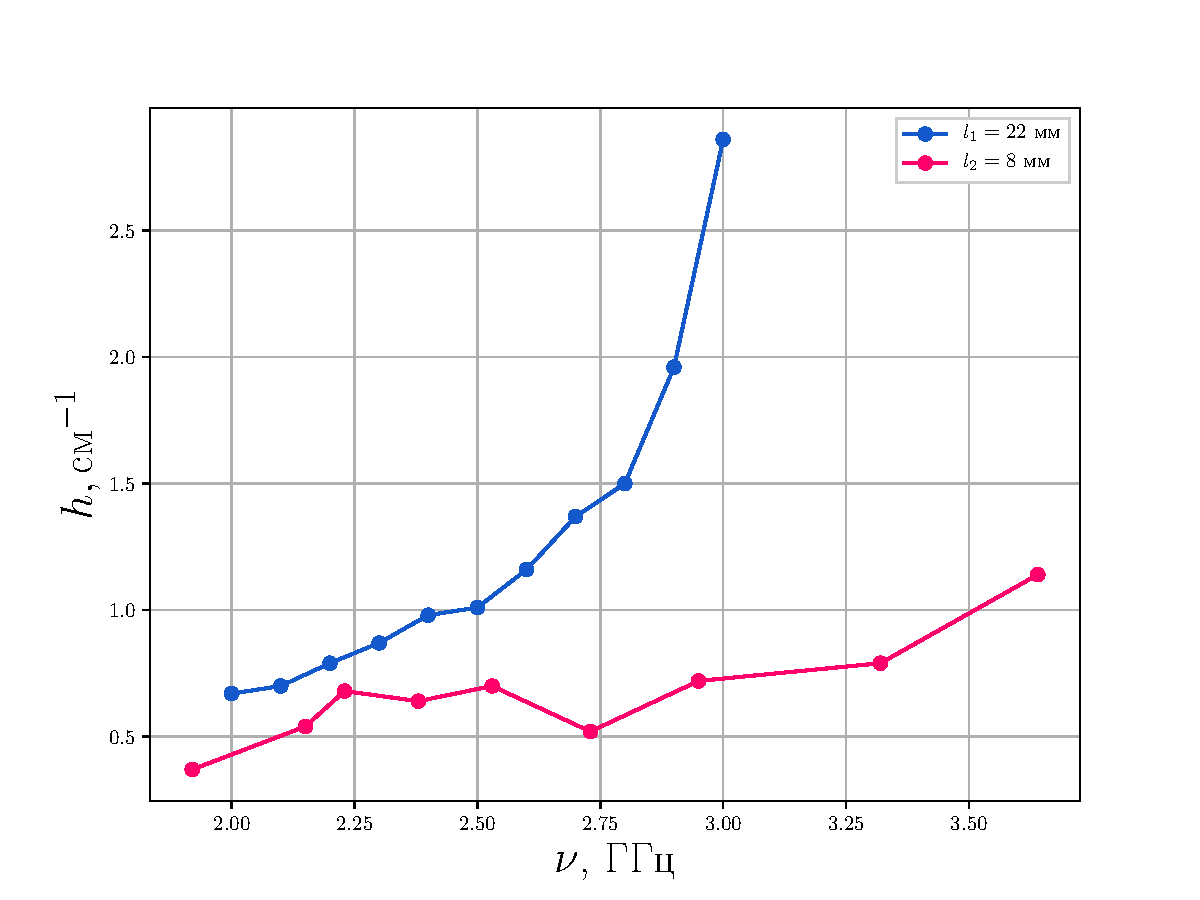
\includegraphics[width=0.9\linewidth]{rec/task1.pdf}
\caption{Дисперсионные характеристики гребенок}
\label{fig:1}
\end{figure}

\subsection*{Задание 2. Продольное распределение поля.} % (fold)
На гребенке 1 было прослежено изменение характера распределения поля вдоль системы с изменением частоты в широких пределах вплоть до частоты запирания: $\omega_{\text{зап}}\sim \frac{c \pi}{2l}$ 
На основе экспериментальных данных (см. рис.\ref{fig:2} ) можно сделать вывод о частоте запирания данной гребенки $\omega_{\text{зап}}\simeq 3100 $ ГГц. 
\begin{figure}[h!]
    \centering
    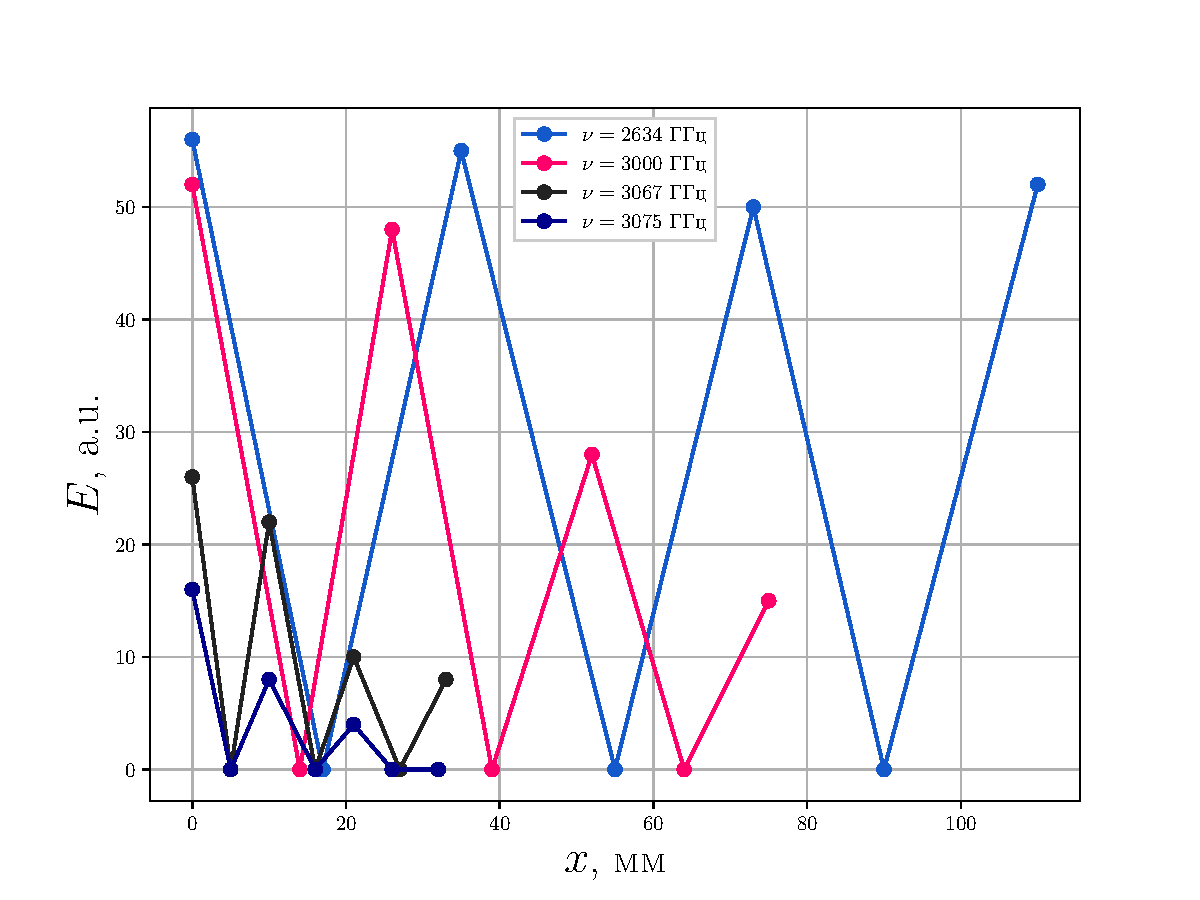
\includegraphics[width=0.9\linewidth]{rec/task2.pdf}
    \caption{Распределение поля вдоль системы}
    \label{fig:2}
\end{figure}

\subsection*{Задание 3. Зависимость поля от положения крышки гребенки.} % (fold)

\end{document}
